\documentclass{article}
\usepackage[utf8]{inputenc}
\usepackage{graphicx}
\usepackage{enumitem}
\usepackage{indentfirst}
\usepackage{array}
\usepackage{listings}
\usepackage{color}

\title{COS 301 - Indoor Mall Navigation SRS document}
\author{Brute Force}
\date{\today}

\begin{document}
	\maketitle
	
	\begin{figure}[!t]
		
\includegraphics{up_logo.png}
	\end{figure}
	\begin{minipage}{0.4\textwidth}
		\begin{flushleft} \large
			\textbf{NAMES:}\\[0.4cm]
			Thomas Honiball\\
			Thabo Ntsoane\\
			Mpho Mashaba\\	
			Munyadziwa Tshisimba\\
			Bandile Dlamini

		\end{flushleft}
	\end{minipage}
	\begin{minipage}{0.4\textwidth}
		\begin{flushright} \large
			\textbf{STUDENT NUMBER:} \\[0.4cm]
		 	15348751\\ 	
		 	15107532\\		
		 	14309999\\		
		 	11034531\\	
		 	14402425
		\end{flushright}
	\end{minipage}

\maketitle

\pagebreak
\tableofcontents
\pagebreak

\section{Introduction}
The scope of the project is to create a fully interactive mall guide of sorts which will allow users to easily find shops as well as act as a shopping companion, providing a list of available specials within a store based on location as well as allowing users to add items to a shopping cart to purchase and have delivered later. This system also aims to replace electronic maps using augmented reality to guide users to a selected store.
\section{Glossary}
    \begin{table}[h]
        \centering
        \begin{tabular}{|p{5cm}|p{5cm}|}
         \hline
            \textbf{Abbreviation} & \textbf{Description}  \\
            \hline
            AR    &   Augmented Reality \\ 
            \hline
            IoT     & Internet Of Things \\ 
            \hline 
            API     & Application Program Interface \\             \hline
            AOA     & Angle of arrival \\
            \hline
            TOA     & Time of arrival \\
            \hline
            QR      & Quality Requirements\\
            \hline
        \end{tabular}
    \end{table}
\section{Domain Model}
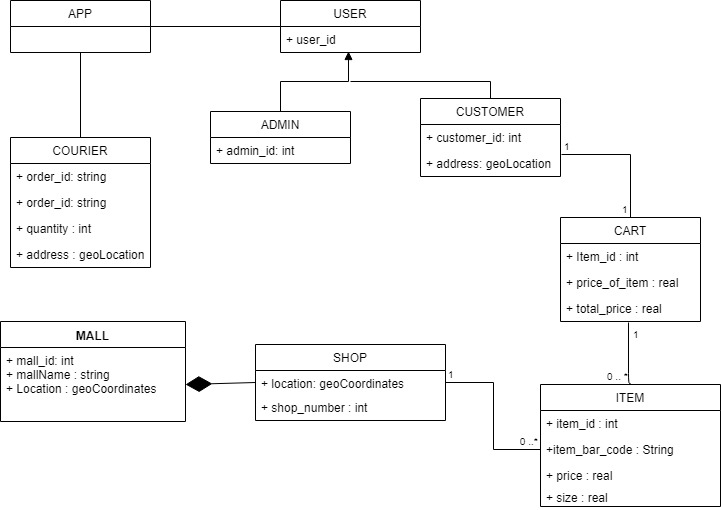
\includegraphics[scale=0.6]{Mall_Navigation.jpg}
\begin{center}
    \textbf{Figure 1: Domain Model}. 
\end{center}
\section{User characteristics}
\subsection{Customer}
This User will interact with the system in order to find a specific shop in a specific mall. The user will be navigated to the specific shop by use of AR. Depending on where the user is in the mall, items on special will be pushed onto the interface for them to see.
\subsection{Maintenance}
This User will update and maintain the system. If there are any shops being moved/renovated or the mall is being extended, this user will make sure that the system is up to date.
\subsection{Delivery Personnel}
This user will interact with the system in order to get the customer order from the shop and deliver it to the given location. This user will use the Google map feature integrated in our system to find the shortest route to the customers location.

\section{Constraints}

\subsection{Battery Life}
\paragraph{Beacon batteries don't last forever so when they die, they will gather no data. Which means that valuable data will be lost.}

\subsection{Costs}
\paragraph{Estimote beacons can be quiet expensive so if we have to cover the entire mall, it will be very expensive.}

\subsection{Range of Beacons} 
\paragraph{The beacons that will be used for this system only have a range of up to a 100 meters. This will be a major problem when when we are dealing with large floors that also have many levels.}

\subsection{GPS Inaccuracy}
\paragraph{Some mobile phones come with app notification features powered by both Geofences and GPS. The challenge here is that GPS can be inaccurate}


\section{Technology Decision}
\subsection{Database & Server Management - Firebase}
\begin{itemize}
    \item We chose Firebase because it provides realtime synchronized data. this means a user can store data with NoSQL cloud Database. when a user goes offline on the app, data remains available across all customers in real time.
    \item Google also provides free Analytic's for mobile apps when using firebase so that the user can see which data is accessed or searched the most so that the developer can modify the app for better user experience.
\end{itemize}

\subsection{Development - Native Android}
\begin{itemize}
    \item We chose Native Android because of it's superior beacon support.
    \item Native Android also ensure speed and agility for mobile Apps with responsiveness and great native app based UI
    \item Native Android applications are more interactive And intuitive. Native mobile apps run much smoother regarding user input and output. These types of apps inherit their devices’ OS interfaces, making them look and feel like an integrated part of the device.
    \item Native Android applications tend to have fewer bugs during development.
\end{itemize}

\subsection{Testing - Travis-CI}
We chose to use Travis Ci for integration because of the following:
\begin{itemize}
    \item It monitors GithHub projects very well.
    \item It easily allows deployment to cloud service
    \item It Runs tests and generates results quickly.
    \item It Easily identifies small and large changes.
\end{itemize}

\section{Functional Requirements}

\subsection{Use cases}

\begin{itemize}
    \item[] UC 1 Create Account \\
     \setlength{\parindent}{24pt}
     \indent UC 1.1 create an account upon purchase or when adding \\ 
     \indent an item to the wish list
     
    \item[] UC 2 Customer Login \\
      \indent UC2.1. Registered users log in using their email and password.
    
    \item[] UC 3 Navigate  \\
     \indent UC 3.1. Navigate to chosen shop \\
     \indent UC 3.2. View current location \\
     \indent UC 3.3. Search for Restrooms. \\
     \indent UC 3.3. Find shortest path
     
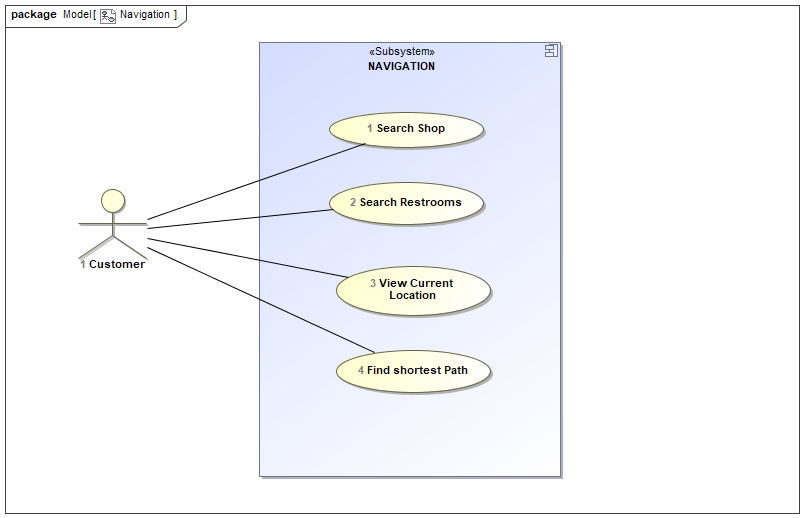
\includegraphics[scale=0.5]{Navigation.jpg}
\begin{center}
    \textbf{Figure 2: Navigation Use Case}. 
\end{center}
     
    \item[] UC 4 Scan Barcode \\
     \indent UC 4.1. Read product name and price from barcode \\
     \indent UC 4.2. Add item to wishlist \\
     \indent UC 4.3. Add item to cart \\
     
    \item[] UC 5 Scan QRcode \\
     \indent UC 5.1. Read product name and price from QRcode \\
     \indent UC 5.2. Add item to wishlist \\
     \indent UC 5.3. Add item to cart \\
    
    \item[] UC 6 Customer Cart \\
     \indent UC 6.1. add an item to cart. \\
     \indent UC 6.2.  remove an item from the cart. \\
     \indent UC 6.3.  checkout \\
     \indent UC 6.3. Payment
     
    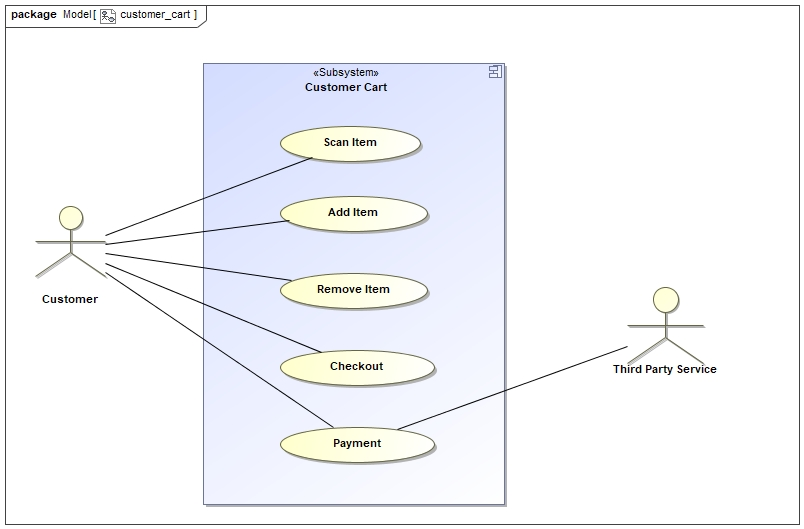
\includegraphics[scale=0.5]{customer_cart.jpg}
    \begin{center}
        \textbf{Figure 3: Customer Cart Use Case}. 
    \end{center}

    \item[] UC 7 Customer Wishlist \\
     \indent UC 7.1.  add an item to wishlist. \\
     \indent UC 7.2.  remove an item from the wishlist. \\
     \indent UC 7.3.  empty the wishlist. \\
     \indent UC 7.4.  move an item from wishlist to cart \\
    
    \item[] UC 8 Delivery \\
     \indent UC 8.1. accept order.\\
     \indent UC 8.2. check delivery status.\\
     \indent UC 8.3. select preferred time range.\\
     \indent UC 8.4. payment
     
    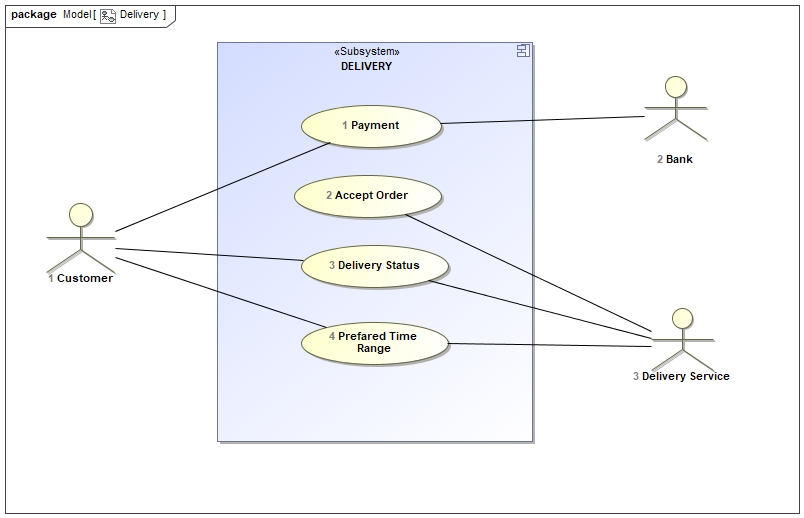
\includegraphics[scale=0.5]{Delivery.jpg}
    \begin{center}
        \textbf{Figure 4: Delivery Use Case}. 
    \end{center}

     \item[] UC 9 Main
\end{itemize}

\subsection{Requirements}
\begin{itemize}
    \item[] \textbf{R1.} A User should be able to navigate to a desired store
     
    \item[] \textbf{R2.} A User should be able to register on the system by creating an account
    
    \item[] \textbf{R3.} A User should be able to log in once registered to view their profile and utilize other functionality.
    
    \item[] \textbf{R4.} A User should be able to view their current location and navigate to a desired location.\\
    \setlength{\parindent}{24pt}
    \indent \textbf{R4.1.} User should be able to search for a store in the mall and\\
    \indent receive the shortest path according to their location\\
    \indent \textbf{R4.2.} User should be able to search for the nearest restrooms\\
    \indent according to their location
    
    \item[] \textbf{R5.} A User should be able to scan the barcode of a product\\ 
    \setlength{\parindent}{24pt}
    \indent \textbf{R5.1.} User should be able to view the product name and price\\
    \indent \textbf{R5.2.} User should be able to add a product to wishlist after\\ \indent scanning barcode\\
    \indent \textbf{R5.3.} User should be able to add a product to cart after\\ \indent scanning barcode
    
    \item[] \textbf{R6.} A User should be able to scan the QRcode of a product\\ 
    \setlength{\parindent}{24pt}
    \indent \textbf{R6.1.} User should be able to view the product name and price\\
    \indent \textbf{R6.2.} User should be able to add a product to wishlist after\\ \indent scanning barcode\\
    \indent \textbf{R6.3.} User should be able to add a product to cart after\\ \indent scanning QRcode
    
    \item[] \textbf{R7.} A User should be able to interact with their shopping cart\\
    \setlength{\parindent}{24pt}
    \indent \textbf{R7.1.} User should be able to add an item from a particular \\
    \indent store\\ 
    \indent to their shopping cart\\
    \indent \textbf{R7.2.} User should be able to remove an item from a particular\\
    \indent store in their shopping cart or clear the entire cart\\
    \indent \textbf{R7.3.} User should be able to edit item specifications from a \\ 
    \indent particular store in their shopping cart\\
    \indent \textbf{R7.4.} User should be able to checkout from the cart 
    
    \item[] \textbf{R8.} A User should be able to interact with their wishlist\\
    \setlength{\parindent}{24pt}
    \indent \textbf{R8.1.} User should be able to add an item from a particular\\ 
    \indent store\\ 
    \indent to their wishlist\\
    \indent \textbf{R8.2.} User should be able to remove an item from a particular\\
    \indent store in their wishlist or clear the entire wishlist\\
    \indent \textbf{R8.3.} User should be able to edit item specifications from a \\
    \indent particular store in their wishlist\\
    \indent \textbf{R8.4.} User should be able to move an item or all times from \\ \indent wishlist to cart 
    
    \item[] \textbf{R9.} A User should be able to have checked out items delivered.\\
    \indent \textbf{R9.1.} User should be able to check their delivery status\\
    
    \item[] \textbf{R10.}The System should allow a CRUD functionality to admin (Maintenance) regarding a Mall's map 
    
\end{itemize}


    
\subsection{Subsystems Traceability Matrix}
    \begin{center}
        \begin{tabular}{ |p{1cm}|>{\centering}p{2.5cm}|>{\centering}p{2cm}|>{\centering}p{2.6cm}|>{\centering}p{2cm}|>{\centering}p{3.3cm}| }
             \hline
              & \textbf{User Account Subsystem} & \textbf{Navigation Subsystem} & \textbf{Shopping Subsystem} & \textbf{Delivery Subsystem} & \textbf{Augmented Reality Subsystem} \tabularnewline
             \hline
             \textbf{R1} & & X & & & \\
             \hline
             \textbf{R2} &X & & & & X\tabularnewline
             \hline
             \textbf{R3} &X & & & & X\tabularnewline
             \hline
             \textbf{R4} & & & & & \\
             \hline
             \textbf{R4.1} & &X & & & \\
             \hline
             \textbf{R4.2} & &X & & & \\
             \hline
             \textbf{R5} & & & & & \\
             \hline
             \textbf{R5.1} & & &X & & \\
             \hline
             \textbf{R5.2} &X & & & & \\
             \hline
             \textbf{R5.3} & & &X & & \\
             \hline
             \textbf{R6} & & & & & \\
             \hline
             \textbf{R6.1} & & &X & & \\
             \hline
             \textbf{R6.2} &X & &X & & \\
             \hline
             \textbf{R6.3} & & &X & & \\
             \hline
             \textbf{R7} & & & & & \\
             \hline
             \textbf{R7.1} & & &X & & \\
             \hline
             \textbf{R7.2} & & &X & & \\
             \hline
             \textbf{R7.3} & & &X & & \\
             \hline
             \textbf{R7.4} & & & X& & \\
             \hline
             \textbf{R8} & & & & & \\
             \hline
             \textbf{R8.1} &X & & & & \\
             \hline
             \textbf{R8.2} &X & & & & \\
             \hline
             \textbf{R8.3} &X & & & & \\
             \hline
             \textbf{R8.4} &X & & & & \\
             \hline
             \textbf{R9} & & & & & \\
             \hline
             \textbf{R9.1} & & & &X & \\
             \hline
             \textbf{R10} & &X & & & \\
             \hline
        \end{tabular}
    \end{center}


\section{Quality Requirements}
    \subsection{Reliability (Q.1)}
    \begin{itemize}
         \item The system should give accurate and precise direction to the user at all times.
        \item The system should retrieve accurate prices and products every time the user scans or is near a specific product.
    \end{itemize}
    
    \subsection{Availability (Q.2)}
    \begin{itemize}
        \item The system should be available for users at most times for navigation. 
    \end{itemize}
    
    \subsection{Security (Q.3)}
    \begin{itemize}
        \item The Application should perform transactions successfully and secure regarding transaction performed on the application.
    \end{itemize}
    
    \subsection{Scalability (Q.4)}
    \begin{itemize}
        \item The application should be able to accommodate a large number of users as they'll be navigating all around different malls.
        \item The application should be able to accommodate large volume of scanning and retrieving items from database for quotes.
    \end{itemize}
    
\section{Architecture and Design}

\subsection{System Type}
\noindent Our system is an event-driven system which relies on various changing states to accomplish use cases. These states are triggered based on certain system properties like device location.

\subsection{System Architecture}
\noindent\textbf{Client-Server:}\\
The system uses a centralised server to ensure all devices remain updated with identical information during usage and allows client applications to remain lightweight.\\\\
\noindent\textbf{Microservices:}\\
Each element of the client system is designed as a modular component that can be added, replaced or removed without affecting the system as a whole. These microservices work hand in hand to satisfy use cases.\\\\
\noindent\textbf{Model-View-Controller:}\\
Each microservice present on the client system makes use of a model in the form of the centralised database, a view to display processed information to the user and a controller to determine the flow of data through the system.\\\\
\noindent\textbf{Object Persistence Framework:}\\
The system as a whole relies on a database to ensure data is not lost between sessions. Certain use cases require that data persists outside of the client's individual usage sessions on the application.

\begin{figure}
    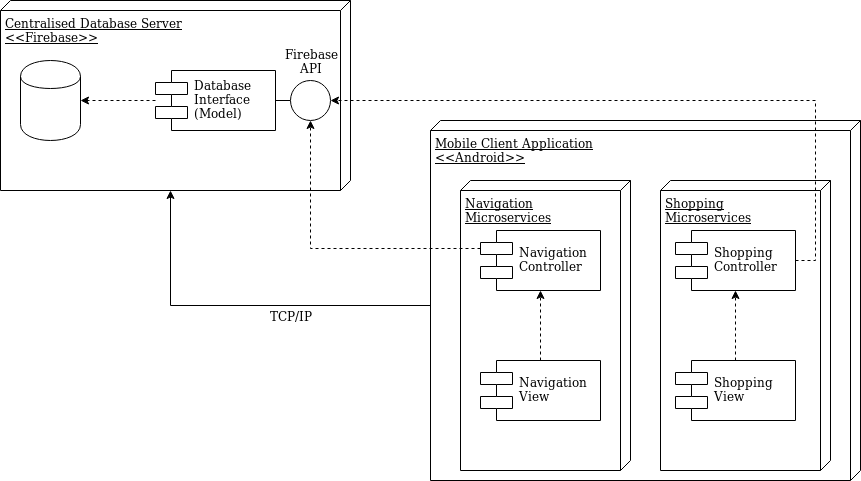
\includegraphics[width=.6\textwidth,left]{deployment_diagram.png}
    \caption{Figure 1: Model}
\end{figure}
\break

\subsection{Non-functional Requirements}
\paragraph{Scalability \\We intend to have a user interface that allows mall owners to add stores to the list as well as supporting expanding maps. \\We plan to use Firebase to ensure that our Database can keep up with the needs of the system.}
\paragraph{ Reliability \\ We intend to use beacons for accurate indoor navigation to specific shops.}
\paragraph{ Availability: \\ We intend to use firebase cloud database hosting and offline synchronization to ensure that the}
    


\section{Trace-ability matrix - Requirements VS Sub-systems}

\begin{center}
        \begin{tabular}{ |p{1cm}|>{\centering}p{2.5cm}|>{\centering}p{2cm}|>{\centering}p{1.9cm}|>{\centering}p{1.9cm}|>{\centering}p{3.3cm}| }
             \hline
              & \textbf{User Account Subsystem} & \textbf{Navigation Subsystem} & \textbf{Shopping Subsystem} & \textbf{Delivery Subsystem} & \textbf{Augmented Reality Subsystem} \tabularnewline
             \hline
             \textbf{R1} & & X & & & \\
             \hline
              \textbf{R2} &X & & & & X\tabularnewline
             \hline
             \textbf{R3} &X & & & & X\tabularnewline
             \hline
             \textbf{R4} & & & & & \\
             \hline
             \textbf{R4.1} & &X & & & \\
             \hline
             \textbf{R4.2} & &X & & & \\
             \hline
             \textbf{R5} & & & & & \\
             \hline
             \textbf{R5.1} & & &X & & \\
             \hline
             \textbf{R5.2} &X & & & & \\
             \hline
             \textbf{R5.3} & & &X & & \\
             \hline
             \textbf{R6} & & & & & \\
             \hline
             \textbf{R6.1} & & &X & & \\
             \hline
             \textbf{R6.2} &X & &X & & \\
             \hline
             \textbf{R6.3} & & &X & & \\
             \hline
             \textbf{R7} & & & & & \\
             \hline
             \textbf{R7.1} & & &X & & \\
             \hline
             \textbf{R7.2} & & &X & & \\
             \hline
             \textbf{R7.3} & & &X & & \\
             \hline
             \textbf{R7.4} & & & X& & \\
             \hline
             \textbf{R8} & & & & & \\
             \hline
             \textbf{R8.1} &X & & & & \\
             \hline
             \textbf{R8.2} &X & & & & \\
             \hline
             \textbf{R8.3} &X & & & & \\
             \hline
             \textbf{R8.4} &X & & & & \\
             \hline
             \textbf{R9} & & & & & \\
             \hline
             \textbf{R9.1} & & & &X & \\
             \hline
             \textbf{R10} & &X & & & \\
             \hline
             \hline
             \textbf{QR}& Q3,Q4 &Q1,Q2 & Q1,Q4 & Q3 & Q1 \tabularnewline
             \hline
        \end{tabular}
    \end{center}

\end{document}
